%
%                       This is a LaTeX 2e version of the
%                       laboratory project template file.
%\documentclass{aa}
\documentclass[a4paper,12pt]{article}
%\usepackage{fullpage,epsf}
%
%                       This subsection generates a title page
%                       Edit only the subsections indicated to put
%                       in the project title, your name, supervisor,
%                       project length in weeks and submission date
\usepackage[english]{babel}
\usepackage[utf8]{inputenc}
\usepackage{csquotes}% Recommended
\usepackage{amsmath,amssymb,latexsym}
\usepackage{graphicx}
\usepackage{subfig}
\usepackage{geometry}
\usepackage{lipsum}
\usepackage{epigraph}

\setlength{\parindent}{2em}
\setlength{\parskip}{1em}
%\usepackage{biblatex}
\usepackage{natbib}
\usepackage{aas_macros}
%\bibliographystyle{agsm}
\usepackage[nottoc,notlof,notlot]{tocbibind} 
\renewcommand\bibname{References}
\bibpunct{(}{)}{;}{a}{}{,} % to follow the 
\usepackage{listings}
\usepackage{color}

\definecolor{dkgreen}{rgb}{0,0.6,0}
\definecolor{gray}{rgb}{0.5,0.5,0.5}
\definecolor{mauve}{rgb}{0.58,0,0.82}

\lstset{
  language=Python,
  aboveskip=3mm,
  belowskip=3mm,
  showstringspaces=false,
  columns=flexible,
  basicstyle={\small\ttfamily},
  numbers=left,
  numberstyle=\tiny\color{gray},
  keywordstyle=\color{blue},
  commentstyle=\color{dkgreen},
  stringstyle=\color{mauve},
  breaklines=true,
  breakatwhitespace=true,
  tabsize=3,
  frame=single
}

\begin{document}
\pagestyle{empty}                       % No numbers of title page                      
%\epsfxsize=40mm                         % Size of crest
\begin{minipage}[b]{110mm}
        {\Huge\bf Computer and \\Information Sciences
        \vspace*{17mm}}
\end{minipage}
\hfill
\begin{minipage}[t]{40mm}               
        \makebox[40mm]{
        
\includegraphics[width=1\linewidth]{strath_logo.png}}
\end{minipage}
\par\noindent                                           % Centre Title, and name
\vspace*{0cm}
\begin{center}
        \Large\bf \Large\bf Dissertation\\
        \Large\bf MSc Software Development\\[10pt]                     % Change to MP/CP/Astro
        \LARGE\bf Automated Mutation Testing for Concurrent Software         % Change to suit
\end{center}
\vspace*{0cm}
\begin{center}
        \bf Patrick Gray\\                           % Replace with your name
        August 2019                                    % Submission Date
\end{center}
\vspace*{5mm}
%
%                       Insert your abstract HERE
%                       
\begin{abstract}

\end{abstract}
\vspace*{2cm}
Signature:\hspace*{8cm}Date: 19/08/2019

\vfill
{\bf Supervisor:} Kostas Liaskos             % Change to suit
\hfill
                                       % Change to suit
\newpage

%
%                       End of Title Page
\pagestyle{plain}                               % Page numbers at bottom
\setcounter{page}{1}                            % Set page number to 1
\tableofcontents                                % Makes Table of Contents

\newpage
\section{Introduction}

\newpage
\section{Background}

The relevant background information required for this project will be presented here, as well as a review of the literature covering concurrent bug patterns and mutation operators. An overview of concurrency in Java and mutation testing for general software will provide the necessary understanding for the motivation of this project.  


\subsection{Concurrency}
\subsubsection{Threads}

Processes are self contained execution environments with private resources; most Java applications only require a single process to run efficiently. Modern computer systems provide multiple cores to process parallel execution of processes. Concurrency utilises this functionality with the use of \textit{Threads}. Threads are light-weight processes that share their resources (memory, open files, etc) with the other threads contained within the process \citep{mois15}. With the advancement of technology producing evermore powerful machines, each individual core has the ability to interleave multiple threads as well as the capability of running threads in parallel on separate cores. 

Creating threads is lighter on resources than creating new processes and the ability to share resources is beneficial to performance. This is the main motivation for using concurrent code; allowing multiple sections of code to run simultaneously for faster execution times. Another positive aspect of this is the improved responsiveness of a system \citep{peierls05}. When one section of a program becomes blocked or slows down, a single threaded system would become unresponsive to the user and would report no information back to explain why. A multi-threaded application would allow a computationally greedy operation to perform in the background without disrupting the rest of the system and remaining responsive to observation and interaction from the user.

Each program has at least one thread, the main thread, created at point of calling the main() method, but subsequent threads can be created after this execution. There are two ways to create new instances of threads. The first is to create an object that has implemented the Runnable interface and pass this to the Thread constructor. The thread will then execute the run() method of the runnable object. The other is to create an object that is a subclass of Thread and executing the run() method pertaining to the object \citep{concurrency19}. In both cases, Thread.start() must be executed to start a specified instance of a thread. Although, threads are not necessarily run in the order of their start() execution, the threads are automatically assigned a priority by the Java Vitrual Machine (JVM), and scheduled in order of highest priority \citep{mois15}. The first instance is a more general and flexible approach since it is implementing the Runnable interface, it allows for the class to inherit functionality from another class. This also has the benefit of allowing its own parameters to be passed to the constructor. The second is easier to use in simple applications, but since it is a subclass of Thread, there are limitations to what the class can do, as only the parent class Thread constructors are available. 

If a thread wants another thread to stop then it can invoke an interruption using Thread.interrupt(), which will throw an exception message to the interrupted thread. A thread can support its own interruption by invoking the sleep() method to stop itself for a specified period of time. After the elapsed time, the thread will resume running, unless an interrupt is called and the thread is terminated. Sleep() can be used by the user to manage the scheduling of threads if it is prescient for a particular operation and limits the unpredictability of the system behaviour. Similar to a thread sleep, Thread.join() can be used for one Thread to wait until another has completed its execution. With no specified time, the Thread may wait indefinitely for the other one to terminate. 


\subsubsection{Atomic Operations} \label{section:atmoic}

An atomic operation is one that is executed and completed all at once or not at all \citep{concurrency19}. It is an action that is considered safe from interference from other operations, as it cannot be stopped during execution and the state of the process cannot be changed by another operation: the state is only affected by the atomic operation from the start to finish. A single line of code does not imply atomicity, no matter how deceptively simple it may appear. For instance, the increment operation for some integer, x++, is actually three separate operations handled by the Java Virtual Machine. First the value of the integer must be fetched, then it is incremented and finally the new value is written back to memory. This may seem trivial, but if mishandled, this can have unexpected and varying results if it is executed in conjunction with another Thread that is accessing the same data. When two threads interleave in such a way, it is referred to as interference. As an example, Thread A and Thread B are tasked to perform the increment operation on x. If they were to run consecutively, allowing for complete execution of the first operation before the initiating the next, the value of x would be expected to have increased by 2. However, if the two operations are executed at the same time, the following scenario could feasibly occur:
\begin{enumerate}
    \item Thread A retrieves the value of x, x = 0.
    \item Thread A increments x, x = 1.
    \item Thread B retrieves the value of x before the Thread A has been given the chance to commit the change of x to memory and thus, x remains equal to 0.
    \item Thread A stores the result of x = 1.
    \item Thread B increments x to 1 and stores the result. Despite two instances of incrementing the value of x, the final value is recorded as 1; the first instance has been overridden by the second.
\end{enumerate}

\begin{table}[]
    \centering
    \begin{tabular}{||l c||} 
     \hline
     Operation & Value of x  \\ 
     \hline\hline
     Thread A retrieves x & 0 \\ 
     \hline
     Thread A increments x & 1  \\
     \hline
     Thread B retrieves x & 0 \\
     \hline
     Thread A stores value of x & 1 \\
     \hline
     Thread B increments x & 1 \\  
     \hline
     Thread B stores value of x & 1 \\
     \hline
    \end{tabular}
    \caption{Example of a non-atomic operation, x++, in two interleaving threads.}
    \label{table:non-atomic}
\end{table}

 

This is only one small example of interference, but similar occurrences of inconsistent memory issues between threads can crop up throughout concurrent systems unless properly managed. Compounding this is the complexity of other scenarios with a greater number of interleaving threads and manipulation of more data. One method of preventing this is utilising the functionality of synchronized code, which will be explored in the following section.


\subsubsection{Synchronization and Locks}
    
Synchronization allows for critical sections of code or methods to be executed atomically with reference to code in other threads. The power of scheduling operations and resource management is passed to the user \citep{silberschatz13}. The synchronized keyword blocks other threads from executing simultaneously during its execution to ensure that the state of the system is only affected by the actions within the synchronized block. Synchronization can be applied to a specific set of actions in a block, specifying the resource to be restricted or to an entire method. The two methods of using the synchronized keyword are shown in Figure \ref{fig:synchronized}. 

\begin{figure}[h]
    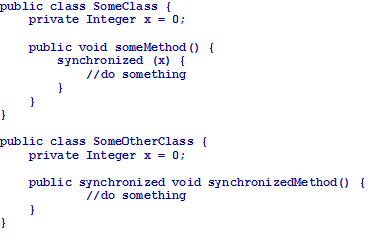
\includegraphics{synchronized.png}
    \caption{Synchronized block and synchronized method}
    \label{fig:synchronized}
\end{figure}

Restricting the whole method will have a more dramatic effect on the performance as no other threads can run concurrently. Applying synchronization to the increment example would solve the observed problem of memory consistency and would guarantee the expected result to occur.

The synchronized keyword achieves the desired affect by imposing a lock on the synchronized block of code that prevents access to the contained object’s fields. After the synchronized block has terminated, the lock is released and normal thread scheduling will resume. Reentrant locks can be used to similar effect to the synchronized keyword, allowing a thread to obtain and release a lock during execution of critical code, much like a synchronized block of code. 

\subsubsection{Liveness}
The liveness of an application expresses its ability to execute without complications in an efficient manner. There are some issues that can interfere with the liveness of an application by slowing it down or even freeze functionality altogether. A deadlock can occur when two threads have locked separate resource, but are waiting on the other thread to release their lock to continue execution. 

\vspace{2pt}
\begin{center}
\noindent Thread 1: locks resource A, waits for resource B
\\Thread 2: locks resource B, waits for resource A 
\end{center}
\vspace{2pt}

In this instance, both resources are locked and unavailable for access until the other is released; the program will perpetually hang in an inescapable catch-22.  


\subsubsection{Executor Service}
Previously, concurrency examples provided have only involved two threads that are relatively simple to follow. In many cases, a program may wish to utilise many more threads for a significant boost in performance. The Java concurrent package offers the Executor Service to help maintain many instances of threads, a thread pool, by abstracting the management and construction of threads from the main program. This can be an invaluable tool for ensuring computation resources are not wasted by the constant creation of new threads for each concurrent action. Instead, a pool of threads is created at once and the threads will wait until they are required. After performing the necessary action, the thread will go back into a state of waiting for a request for work. The size of the pool has a specified limit, to prevent a runaway of thread creation; when all the threads in a pool are currently in use, the executor server will wait to assign work to the next available thread. Creating a thread takes up time and resources, it is far more efficient to recycle previously used threads. 


\subsection{Mutation Testing}
Mutation testing is the process of seeding errors throughout a system’s codebase, to observe the effecting behaviour and evaluate the effectiveness of the present testing coverage \citep{adrion81}. A \textit{mutation operator} is a generalised rule, which describes the changes that will be made to a specific segment of code. The result of applying an operator to a code segment is known as a \textit{mutant} \citep{ammann17}. The premise of mutation testing is simple: if the previously implemented software tests have been designed adequately, then they should recognise the changes to the system behaviour and certain tests should fail accordingly. The mutation is referred to as killed in this instance. This is the ideal outcome when a mutation is applied to a system, as it suggests that the tests have been designed effectively and the coverage is sufficient. However, if a mutation survives by circumventing the tests, this indicates that the tests are either flawed or the test coverage has gaps and not all of the behaviour has been accounted for. This is a useful tool for highlighting weaknesses in test coverage; a full suite of unit tests that successfully pass when run on a system only informs the user that those specific function behaviours are expected. Although it provides no information on the behaviours that have been missed. Mutation testing aides identifying these areas of code that have been overlooked by applying many different mutations throughout the whole system, which should disrupt as much expected behaviour as possible. Thus, when a mutation is not successfully killed by any unit test, the location of the altered code will indicate that there is improvement to be made in the test coverage related to the affected area.

One example of a renowned mutation testing tool is Pitest (PIT), which combines traditional line coverage with mutation coverage, to offer a comprehensive and fast testing environment for Java applications \citep{pit19}. The list of mutation operators it provides is extensive, covering relational operators (e.g. \textless, \textless=, \textgreater, \textgreater=), mathematical operators (e.g. +, -, *, etc.), logic statements a variety of different common method calls and return values \citep{pit19}. A mutation usually consists of altering a small section of code or removing a section entirely. For example, a conditional boundary operator would make the following mutation  in Figure \ref{fig:mutation}. 

\begin{figure}[h]
    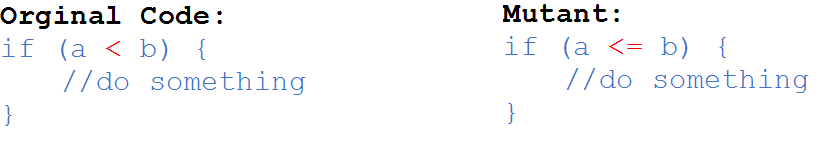
\includegraphics{mutation.png}
    \caption{Relational operator mutation}
    \label{fig:mutation}
\end{figure}
    
The code now has a slightly different meaning. Designing effective unit tests involves specifically testing code at such boundary cases. The behaviour of the code would be monitored for values of a when less than b, equal to b and greater than b, with a separate test for each scenario. Prior to the mutation, the if statement would not be executed during runtime for when a is equal to b, but after the mutation the if statement would be entered. Thus, a unit test that previously would pass for this scenario should fail due to the alteration and the mutation could be considered successfully killed. PIT will apply many of these mutations on the byte code generated after compilation, instead of on the source files. This produces significantly faster runtimes. After mutation, PIT will automatically run the new java files against the designated unit tests and produce a set of results detailing the fates of each mutation. The varying states explained below:

\begin{description}
    \item[Killed - ]The mutation was successfully discovered by the presence of a failed unit test.
    \item[Lived -]The mutation was unsuccessfully discovered with no failed unit tests. 
    \item[No coverage -]The mutation lived because of a lack of unit tests covering the relevant mutated section of code. 
    \item[Non-viable -]The mutation affected the Java bytecode such that the JVM could not load the file.
    \item[Timed out -]The mutation created an infinite loop so execution of the file could not terminate. 
    \item[Memory error -]The mutation increased “the amount of memory used by the system or the result of the additional memory overhead required to repeatedly run your tests”.
    \item[Run error -]The mutation caused the file to be unable to run, similar to non-viable mutations.
\end{description}

The results detail which mutations were applied, identify which tests managed to kill mutations and produce the ratio of successfully caught mutations to the total number of seeded errors. Although PIT offers a wide range of mutation operators, it is lacking in support for concurrent systems. Performing unit tests on multi-threaded code is not as straightforward as single threaded [unclear why].


\subsection{Regular Expressions}    

The theory of mutation testing has been presented, however the mechanism by which mutations are applied is not a simple process with a single approach. The method used in this project is a high-level approach, utilising regular expressions to identify and manipulate strings. This is a different approach to the method seen in the Pitest mutation tool; a more sophisticated and technically complex method operating on bytecode. For the size and scope of this project, performance is less of a concern, so manipulating source code is a viable option. 

Regular expressions, regex for short, are a syntactic description of a pattern, often used to search or manipulate strings in a text [cite]. Exact strings can be found with ease, but the true power behind regular expressions is the ability to search for generic patterns and manipulate any matches returned. The java.util.regex package allows a user defined pattern to be interpreted and will find any matches within a given text. This is primarily achieved using the Pattern and Matcher classes. Inputting a regular expression into a Pattern as a parameter will create a compiled version of the regex. The syntax of a pattern is built up of special character constructs that can match with independent characters or a defined range of characters. For example, a regex pattern could be used to search for a date in the following format DD month YYYY, i.e. 20 July 1969. This format has strict rules specifying that a date must consist of two digits followed by a word and finally four more digits. The regex can be made more complex by imposing more rules limiting the range of numbers for the day section to be between 1-31; the month section to only consist of the exact strings for the calendar months and the year section to be greater than 0000. All of this is achievable with the Java regex package. However, to keep it simple, the following regex example will only look for the basic two digits-word-two digits:
\begin{equation}
    (\setminus d\{2\}) (\setminus s) ([a-zA-Z]+) (\setminus s) (\setminus d\{4\})
\end{equation}

\begin{description}
    \item[ $\setminus d\{2\}, \setminus d\{4\}$ -] exactly 2 or 4 digits, respectively
    \item[ $\setminus s $ -] a single whitespace character
    \item $[a-zA-Z]+$ - one or more letters in the range of a to z, lower or upper case
\end{description}

The brackets separates the regex into groups that can be manipulated in isolation from the rest of the matched expression. A Matcher object can then be created to compare a character sequence against the pattern and return any matches. The find() method attempts to find the next matching sequence in the input. The group(int group) method returns the sequence that was matched by the specified group, identified in order of appearance in the regex, e.g. ([a-zA-Z]+) is group 3. Finally, if the user wishes to replace any part of a matched string, the replaceFirst(String replacement) and replaceAll(String replacement) methods will replace either the first matched substring or all matching substrings, respectively, with a specified replacement string. A full API for these classes is provided by \citeauthor{regex_package19}.


\subsection{Concurrent Bug Patterns}

During the software development life cycle, it is vitally important to contribute a significant portion of effort into the architectural design of the software. A well designed system will provide a solid foundation in avoiding unforeseen faults throughout development. \citeauthor{farchi03} present a systematic approach to preventing certain concurrency related errors in their research on Concurrent Bug Patterns \citep{farchi03}. \textit{“Design patterns are solutions to recurring problems in a given context. A design pattern accentuates the positive, i.e., how to solve a recurring problem well.”} 

This is a general concept, originally used to describe physical construction, but is equally applicable to software development \citep{gamma15}. However, poor design patterns can have the reverse effect and introduce their own set of errors. This gives rise to what is known as a bug pattern: \textit{“A bug pattern is an abstraction of a recurring bug. In other words, a bug pattern is a literary form that describes a commonly occurring error in the implementation of the software design.”}

By identifying common concurrency errors made by developers, \citeauthor{farchi03} have categorised a variety of different bug patterns. In their systematic approach, they offer a more technical definition of a bug pattern in a program, P, relating to potential number of interleavings between threads in a concurrent system, I(P), and the maximum number of interleavings the system can have whilst remaining correct, C(P). A concurrent bug pattern can be found within the range I(P) – C(P) \citeauthor{farchi03}. Typically, bugs will occur due to a faulty assumption by the developer, separated into the following three categories: 

\begin{enumerate}
    \item "A code segment is mistakenly assumed to be undisturbed, implicitly or explicitly, by other threads;
    \item As a result of the mistaken assumption that a certain execution order of concurrent events is impossible;
    \item When a code segment is mistakenly assumed to be nonblocking.”, \citep{farchi03}.
\end{enumerate}

Farchi et al. provide many examples in each category, but only the relevant bug patterns will be explored in the following sections, separated into the categories defined above. Due to the limited scope of the concurrent systems sampled in this project, instances of many concurrent keywords are not present, meaning that some bug patterns are not available for exploration. All the bug patterns that have the potential to be found are presented here.        

    
\subsubsection{Unprotected Code}
Concurrent code can be considered to be protected when only a single thread is executing a concurrent event between the first and last events in the code segment. When multiple threads begin executing concurrent code simultaneously, errors are bound to arise.   

\textbf{\\Nonatomic Operations Assumed to be Atomic Bug Pattern} 
\\This bug relates to the example in Section \ref{section:atmoic}, wherein a developer falsely assumes that a fragment of code is an atomic operation and therefore protected. On a surface level, a code fragment may appear to be executed as a single operation, but the bytecode translation consists of more operations.

\textbf{\\Two-Stage Access Bug Pattern}
\\Consider a sequence of concurrent actions, it can be insufficient to protect the separate operations individually. The example provided by \citeauthor{farchi03} is as follows: \textit{“Adding and removing operations to some data base are performed concurrently by first accessing a table to translate from key1 to key2. Then key2 is used to access another table and add or remove the data. Accesses to both tables are synchronized.”}, \citep{farchi03}. Despite both processes being synchronized, there is a gap in protection between the first and second table access. Consequently, the tables are open to access from other threads during this window that allows for unwanted changes to the data.

\textbf{\\Wrong Lock or No Lock Bug Pattern}
\\This pattern can occur when one thread has locked an action but other threads attempt to acquire a different lock for a concurrent action. The other threads will either successfully obtain the wrong lock or don’t obtain any lock. Thus, the code is unprotected and susceptible to interference from interleaving threads.


\subsubsection{Unexpected Interleavings}

In these scenarios, the programmer has assumed an interleaving between threads to be impossible, often due to considering the computation time of a certain action to be fast enough that it will not overlap with another concurrent action. Generally, this is considered bad practice as it is often difficult to predict the length of time for a process to complete, which can also vary between executions. 

\textbf{\\Sleep() Bug Pattern}
\\A programmer might understandably attempt to control the scheduling of thread execution by introducing delays, utilising the sleep() method, and specifying a time they have deemed to be sufficient for complete execution of certain critical sections. Instead, the join() method would be more appropriate in this circumstance.

\citeauthor{farchi03} cover another example of an unexpected interleaving bug pattern involving the notify() and wait() methods. However, the concurrent systems tested in this project do not contain any instances of these methods and thus, the notify() bug pattern will not be covered in this review.   


\subsubsection{Blocking Code}

In some circumstances, a segment of code can have an unexpected behaviour in a thread that blocks other threads from executing, resulting in the system hanging indeterminately. This obviously can have a very drastic effect on the performance of a program.

\textbf{\\Blocking Critical Section Bug Pattern}
\\After execution of a critical section in a thread is complete, it is expected to relinquish control and allow other threads to execute. If the correct procedure for this has been overlooked then other threads are left waiting for the first thread to terminate; an event which may never happen.   

Again, only one of the patterns in this category can be found in the concurrent systems and is covered in this section.

    
\subsection{Mutation Operators}
\citet{bradbury06} have comprehensively designed a set of mutation operators specific to the concurrent functionality and the bug patterns identified by \citeauthor{farchi03} The focus of their research is in response to the updated concurrent functionality introduced in the J2SE 5.0 version of Java. Synchronization can now be implemented using explicit locks, semaphores, barriers, latches and exchangers. Support for these various concurrent operations persists through the more recent versions of Java with some minor updates and revisions. In total, \citeauthor{bradbury06} to produce 22 different mutation operators, each of which are associated with a number of different concurrent methods. The operators are split into groups relating to the concurrent bug patterns described in the work of \citeauthor{farchi03}

Mutation analysis for non-concurrent systems has been covered extensively in research and made available through a variety of different tools [cite]. With their mutation operators, \citeauthor{bradbury06}'s aim is to help improve the quality and development of concurrent Java applications by making programmers aware of the various pitfalls surrounding concurrency. The operators have been divided into five categories:
\textit{
\begin{enumerate}
    \item "Modify parameters of concurrent methods
    \item Modify the occurrence of concurrency method calls (removing, replacing and exchanging)
    \item Modify keywords (addition and removal)
    \item Switch concurrent objects
    \item Modify critical regions (shift, expand, shrink and split)" \citep{bradbury06}
\end{enumerate}
} 

Some of these operators are modified versions of existing operators, whereas some are novel. 1-3 of the above categories will be explored in the following sections. Categories 4 \& 5 are not covered since none of the mutation operators from these categories are implemented in the tool developed for this project. The specific operators that have been implemented will be fully explored in the Methodology section of this report. The full list of \citeauthor{bradbury06}'s mutation operators can be found in Table \ref{table:MO_cat} in the Appendices section.


\subsubsection{Modify Parameters of Concurrent Method} \label{Modify Parameters}

Altering the parameters of a method in any way can cause a dramatic difference to the original intention when calling the method. The operators in this category aim to do just that for any concurrent method or methods related to threads. This can involve changing the value of an input parameter or removing a parameter altogether, assuming the method has an overloaded version to support this removal.  


\subsubsection{Modify the Occurrence of Concurrency Method Calls} \label{Modify Method Calls}

In contrast to the previous category of modifying method parameters, this set operates on the method calls themselves. The mutation can manifest in three forms: a method call can be removed, replaced or exchanged with a similar method.   


\subsubsection{Modify Keywords} \label{Modify Keywords}

This category is similar to the previous type, but focuses solely on the addition or removal of certain concurrent keywords, such as static, synchronized, volatile and finally. These keywords affect the behaviour of classes, methods and variables, thus modifying them may have significant effects when calling a mutant version.


\subsection{Motivation}

The background information has been presented and the literature surrounding Mutation testing operators has been explored. The motivation for the project should now be clear. Although there are mutation testing tools available for Java applications, they lack support for concurrency. Thus, the aim of the project is to build a mutation testing tool that will automatically apply mutations specific to concurrent operations, utilising the operators provided by \citeauthor{bradbury06} This will provide support for programmers to analyse the effectiveness of their unit tests for multi-threaded functionality.

The following Methodology section will describe the development process in detail and the steps taken to ensure the mutation testing tool is robust.   



\newpage
\section{Methodology}
\subsection{Mutation Operators}


\subsubsection{MXT - Modify Method-X Timeout}

The MXT operator falls under the category of \textit{Modify Parameters of Concurrent Method}, found in Section \ref{Modify Parameters}. The objective of this operator is to modify the time parameter in the methods wait(long time), await(long time), sleep(long time) and join(long time) \citep{bradbury06}. The wait, await and join methods both have an overloaded equivalent without the time parameter, meaning that the mutation can remove or modify for varying effects. Removing the time parameter from the wait method forces the current thread to remain inactive until a notify() or notifyAll() method is called to release the interruption. The await method is similar to the wait method, but is instead released by a signal() or signalAll() method call in another thread. The join method is called on a thread and will wait until it has completed execution or until the specified time has elapsed, after which, the code following the join() call will be executed in the same thread. The sleep method will interrupt the current thread for the specified time. The mutation that has been implemented in the tool is to either remove the time parameter, if applicable, or to reduce the time by half.        


\subsubsection{MSP - Modify Synchronized Block Parameter}
	
	

\subsubsection{RTXC - Remove Thread Method-X Call}


\subsubsection{RCXC - Remove Concurrency Mechanism Method-X Call}
	
	
	\subsection{Mutation Tool}
	\subsection{Concurrent Software}
	    \subsubsection{Banking System}
	    \subsubsection{Incrementer System}
	\subsection{Unit Tests}
	    \subsubsection{JUnit Tests}
	    \subsubsection{Concurrent Tests}
    \subsection{Software Engineering}
	
	
\newpage	
\section{Analysis}
    \subsection{Results}
    

\subsection{Results Analysis}

Bradbury et al. conjecture that “The MXT operator with the sleep() and join() methods is most likely to result in the sleep() bug pattern… where a sleep() or join() is used by a caller thread to wait for another thread, reducing the time may cause the caller thread to not wait long enough for the other thread to complete.  

“The MXT operator when applied to an await method call will most likely result in an interference bug” – compare actual results to their hypotheses.

“The MSP operator will result in the wrong lock bug pattern”

“The ESP mutation operator can result in a wrong lock bug because exchanging two adjacent locks will cause the locks to be acquired at incorrect times for incorrect critical regions. The ESP operator can also cause a classic deadlock (via deadly embrace) bug to occur as is the case in the above example.”

“Removing the wait() method can cause potential interference, removing the join() and sleep() methods can cause the sleep() bug pattern, and removing the notify() and notifyAll() method calls is an example of losing a notify bug.”

“The RCXC operator removes this [unlock] call thus the lock is not released. This is an example of a blocking critical section bug.”

    
    
    
    
\subsection{Methodology Analysis}

The automatic mutation application tool currently only supports application of four of these mutation operators with all of the relevant concurrent keywords and methods: MXT, MSP, RTXC and RCXC. However, at least 7 more of the operators could be implemented with little difficulty due their similar mechanisms. The regular expression used is very consistent for simple removals of keywords and minor modifications to method parameters. The operators that have been implemented already were chosen based on the needs of the banking system and the limited number of concurrent methods present in the code.   

The incrementer system has been designed to purposefully encounter concurrent problems, such as thread interference and memory consistency errors. The reason behind this is to easily catch the bugs that are present after a mutation has taken place in one of the system class files. Await() and sleep() statements were utilised to slow down the computation time and increase the likelihood of two threads attempting to access state variables within the same window. This serves as a proof of concept that it is possible and fairly straightforward to design effective unit tests for concurrent code. Although, obviously, in real-life scenarios, compromising the performance and execution time of large systems is not ideal. Especially considering the main motivation of implementing concurrency to a system is to improve the performance. The test environment can be used to determine whether the system has been properly safeguarded with less concern for efficiency.

There may be an argument to introduce a default wait time of 0 seconds, stored as a variable, to be used as a parameter for the relevant methods, so that in normal use the system will function with the desired efficiency. However, when it comes to testing, this variable can be altered to a more suitable value that will provide significant opportunity for errors to arise that would remain hidden in the default state of execution. 

It was deemed sufficient to test the systems with only two threads. Since the systems were small in scale and designed in such a manner that errors would be readily caught, increasing the number of threads would be superfluous. If a mutation was identified and killed by any unit test with only two interleaving threads, then the mutation would definitely be caught in number of more threads. However, in larger, more complex systems, any bug may be significantly harder to find, so increasing the number of threads with the objective of maximising the likelihood of interference could be an effective approach.

    
    
\newpage	
\section{Conclusion}

\subsection{Future Work}
The original goal was to end up with a full test suite that would seed many mutations throughout the code, perform the unit tests and produce a set of results. The results would detail which mutations were applied, identify which tests managed to kill mutations and produce the ratio of successfully caught mutations to the total number of seeded errors. Due to time limitations, a revision of expectations and priorities, the focus was on developing the mutation system and the unit tests for the sample test systems. Thus, many of the stages above were carried out manually. A complete automatic tool for evaluating the effectiveness of concurrent tests would be a valued area for future development. The inspiration for the tool described was spawned from the presence of other mutation testing tools, such as Pitest, which provides a full mutation testing environment and many operators to select. However, none of the available tools provide support for concurrent operators due to the special difficulties that surround the subject.
    
\newpage
\section{Acknowledgements}

\bibliographystyle{apa} % style aa.bst
\bibliography{bibliography.bib}

\newpage
\appendix

\section{Appendices}
\begin{table}
    \centering
    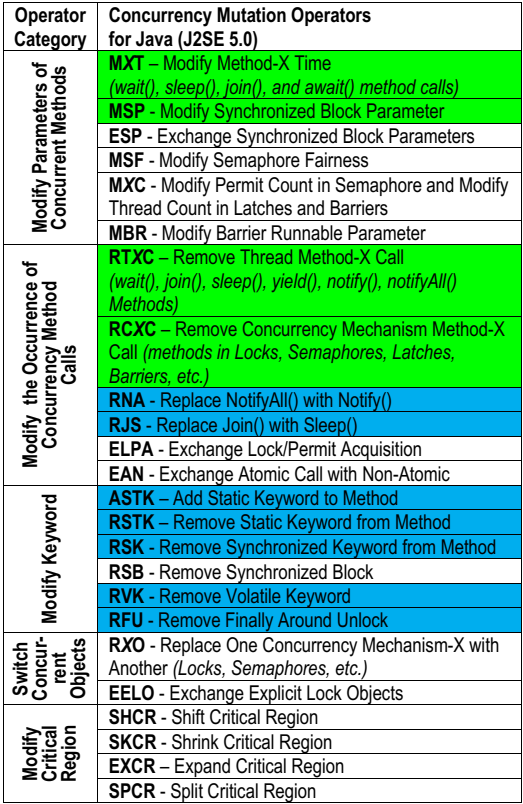
\includegraphics[scale = 0.9]{MO_categories.png}
    \caption{List of concurrency mutation operators devised by \citeauthor{bradbury06} The green highlighted operators have been fully implemented in the mutation testing tool. The blue highlighted operators could be implemented without difficulty.}
    \label{table:MO_cat}
\end{table}

\begin{table}
    \centering
    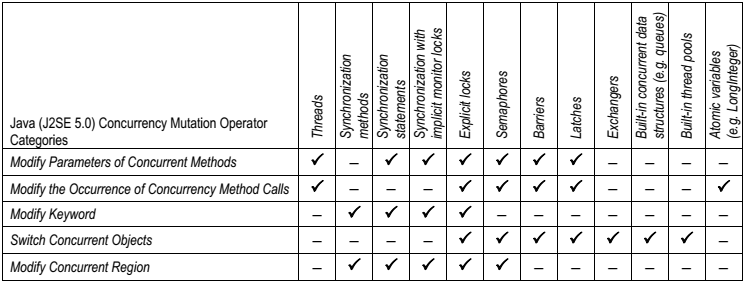
\includegraphics[scale = 0.85]{MO_features.png}
    \caption{The relationship between new mutation operators for concurrency and the concurrency features provided by J2SE 5.0 \citep{farchi03}.}
    \label{table:MO_features}
\end{table}


\end{document}
